\documentclass[aspectratio=169,12pt]{beamer}

% ===== 主题 =====
\usetheme{metropolis}
\usepackage[UTF8, fontset=none]{ctex}
\usepackage{amsmath}
\usepackage{amssymb}
\usepackage{graphicx}
\usepackage{booktabs}
\usepackage{multirow}
\usepackage{tikz}
\usetikzlibrary{shapes,arrows,positioning}
\usepackage{caption}
\usepackage{appendixnumberbeamer}

% ===== 字体（与论文一致）=====
\setCJKmainfont{simsun.ttc}[Path=fonts/, AutoFakeBold=3]
\setCJKsansfont{simhei.ttf}[Path=fonts/, AutoFakeBold=3]
\setCJKmonofont{simsun.ttc}[Path=fonts/, AutoFakeBold=3]
\setCJKfamilyfont{heiti}{simhei.ttf}[Path=fonts/, AutoFakeBold=2]
\setCJKfamilyfont{songbold}{simsun.ttc}[Path=fonts/, AutoFakeBold=2]
\newcommand{\heiti}{\CJKfamily{heiti}}
\newcommand{\songti}{\CJKfamily{\CJKrmdefault}}
\setmainfont{times.ttf}[
    BoldFont=timesbd.ttf, ItalicFont=timesi.ttf, BoldItalicFont=timesbi.ttf,
    Path=fonts/]

% 正文使用宋体（beamer 默认 sans，强制切换为 rmfamily），粗体用仿粗而非黑体
\setbeamerfont{normal text}{family=\rmfamily}

\xeCJKsetup{PunctStyle=quanjiao}

% ===== 配色 =====
\definecolor{mDarkTeal}{HTML}{23373b}
\definecolor{mLightBrown}{HTML}{EB811B}
\definecolor{mLightGreen}{HTML}{14B03D}
\setbeamercolor{frametitle}{bg=mDarkTeal}
\setbeamercolor{progress bar}{fg=mLightBrown}
\setbeamercolor{alerted text}{fg=mLightBrown}

% ===== 图表标题 =====
\captionsetup{font=small, labelfont=bf, labelsep=space, justification=centering, skip=4pt}

% ===== 元信息 =====
\title{基于机器学习方法的水库滑坡位移预测及预警研究}
\subtitle{——以藕塘滑坡为例}
\author{答辩人：韦承谦 \quad 指导教师：陈铭熙}
\institute{}
\date{\vspace{1.5em}2026年5月22日}

\begin{document}

% ============================================================
% 1. 封面
% ============================================================
\maketitle

% ============================================================
% 2. 研究背景与工程概况
% ============================================================
\begin{frame}{研究背景}
  \textbf{问题背景}
  \begin{itemize}
    \item 三峡库区水库滑坡受\alert{库水位周期涨落}与\alert{季节性降雨}耦合驱动，呈典型\textbf{阶跃型}变形特征
    \item 传统确定性点预测难以量化风险可信度，单一阈值预警缺乏适应性
  \end{itemize}
  \vspace{0.6em}
  \textbf{研究目标}
  \begin{itemize}
    \item 构建``特征分析—位移预测—概率预警''机器学习框架
    \item 以三峡库区典型阶跃型滑坡——藕塘滑坡为案例进行系统验证
  \end{itemize}
\end{frame}

% ============================================================
% 3. 藕塘滑坡概况
% ============================================================
\begin{frame}{藕塘滑坡概况}
  \begin{columns}[T]
    \begin{column}{0.42\textwidth}
      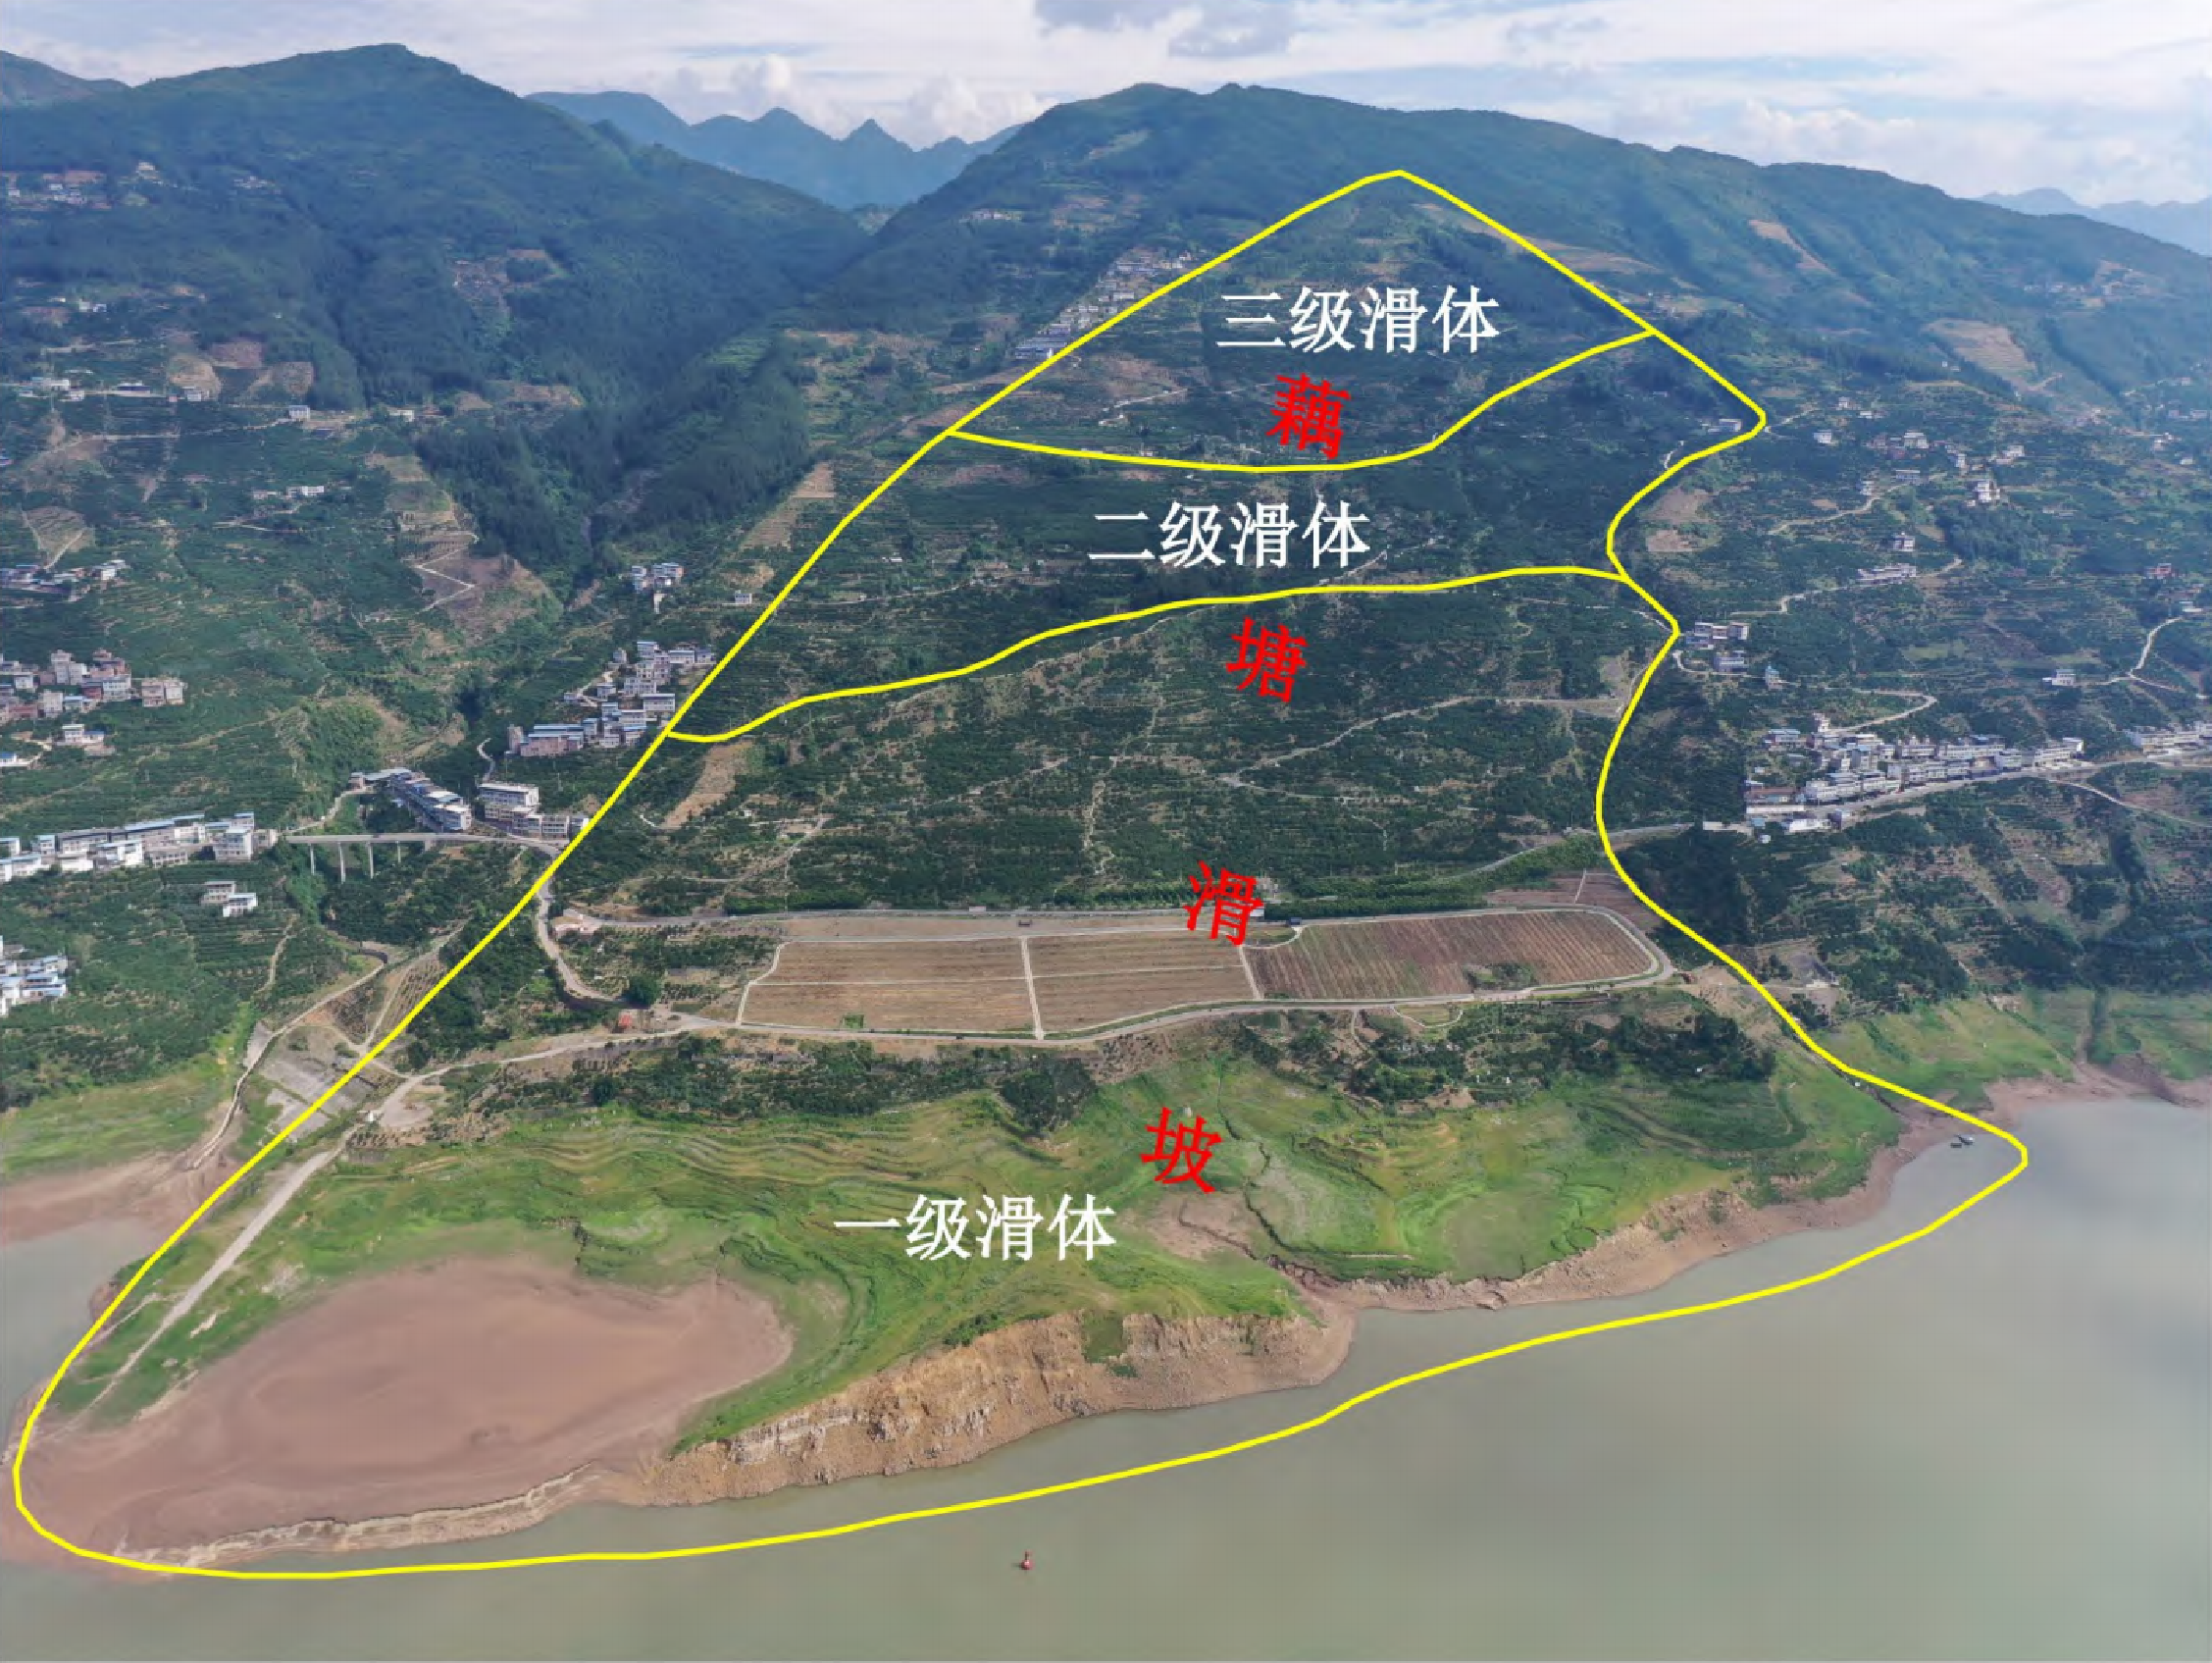
\includegraphics[width=\textwidth,height=0.45\textheight,keepaspectratio]{figures/chapter2/Panoramic_map_of_Outang_landslide.pdf}
      \vspace{0.8em}
      \textbf{基本特征}
      \begin{itemize}
        \item 重庆市奉节县安坪镇，长江南岸
        \item 体积约 $9\times10^7\,\text{m}^3$，最大厚度 114\,m
        \item 三个子区，多期次复合滑动
        \item 软弱夹层控制变形，遇水软化显著
      \end{itemize}
    \end{column}
    \begin{column}{0.54\textwidth}
      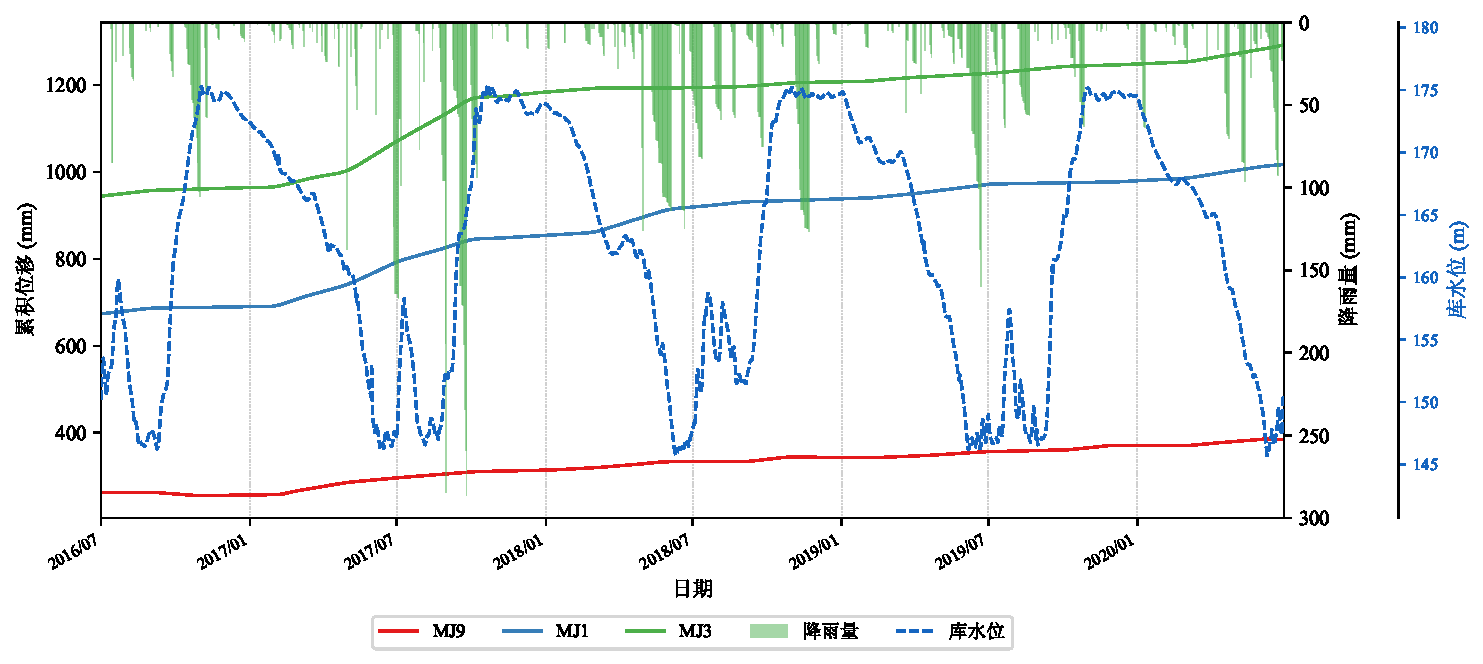
\includegraphics[width=\textwidth,height=0.45\textheight,keepaspectratio]{figures/chapter2/monitoring_data_overview.pdf}
      \vspace{0.8em}
      \textbf{监测数据}
      \begin{itemize}
        \item 时间：2016年7月—2020年6月（4年，1457条日尺度记录）
        \item GNSS 位移：MJ1（中部）、MJ3（中后部）、MJ9（后缘）
        \item 地下水、库水位、降雨、气象要素同步采集
      \end{itemize}
    \end{column}
  \end{columns}
\end{frame}

% ============================================================
% 4. 技术路线
% ============================================================
\begin{frame}{技术路线}
  \centering
  \vspace{1em}
  \begin{tikzpicture}[
    node distance=1.2cm,
    box/.style={rectangle, draw=black, fill=blue!20, rounded corners=4pt,
                text centered, minimum width=6cm, minimum height=0.9cm,
                font=\bfseries\small, inner sep=6pt},
    arr/.style={->, >=stealth, thick, draw=black!60},
  ]
  \node[box, fill=blue!30] (p1) {特征分析（LightGBM + SHAP）};
  \node[box, fill=blue!20, below=of p1] (p2) {位移预测（LSTM）};
  \node[box, fill=blue!10, below=of p2] (p3) {概率预警（$V_0$ 四级体系）};
  \draw[arr] (p1) -- (p2);
  \draw[arr] (p2) -- (p3);
  \end{tikzpicture}
  \vspace{1em}
  \begin{block}{核心思路}
    \centering
    多源监测数据 $\to$ 可解释特征筛选 $\to$ 多监测点 LSTM 预测 $\to$ 概率分布映射四级预警
  \end{block}
\end{frame}

% ============================================================
% 5. 特征分析：LightGBM + SHAP
% ============================================================
\begin{frame}{特征分析：LightGBM + SHAP}
  \begin{columns}[T]
    \begin{column}{0.50\textwidth}
      \textbf{方法}
      \begin{itemize}
        \item LightGBM：高效梯度提升树，直方图算法 + Leaf-wise 生长策略
        \item SHAP：基于博弈论的特征归因，量化各因子贡献度
        \item 5折时序交叉验证 + SMOTE 过采样
        \item 5天滑动窗口构建候选特征
      \end{itemize}
    \end{column}
    \begin{column}{0.46\textwidth}
      \textbf{关键发现}
      \begin{enumerate}
        \item 历史位移累积与库水位为\textbf{主控因子}
        \item 降雨、地下水位次之，气象要素贡献最小
        \item 时滞窗口：库水位 7--14 天，降雨 3--7 天
        \item 库水位下降 + 强降雨耦合时预警概率显著增加
      \end{enumerate}
    \end{column}
  \end{columns}
  \vspace{0.5em}
  \begin{alertblock}{模型性能}
    回归 MSE：$0.0780 \pm 0.0641$；分类 AUC：$0.6795 \pm 0.1181$，召回率 76.23\%
  \end{alertblock}
\end{frame}

% ============================================================
% 6. LSTM 位移预测模型
% ============================================================
\begin{frame}{LSTM 位移预测模型}
  \begin{columns}[T]
    \begin{column}{0.48\textwidth}
      \textbf{模型设计}
      \begin{itemize}
        \item 输入：MJ9、MJ1、MJ3、ATU4 四点历史位移序列
        \item 利用滑坡体空间协同变形特征进行联合预测
        \item 2层 LSTM（25→15 隐含单元）+ Dropout
        \item Adam 优化器，MSE 损失，MinMax 归一化
      \end{itemize}
      \vspace{0.5em}
      \textbf{概率预测策略}
      \begin{itemize}
        \item \alert{50 次独立随机初始化训练}
        \item 收集预测统计分布，构建分位数预测区间
        \item 量化认知不确定性
      \end{itemize}
    \end{column}
    \begin{column}{0.48\textwidth}
      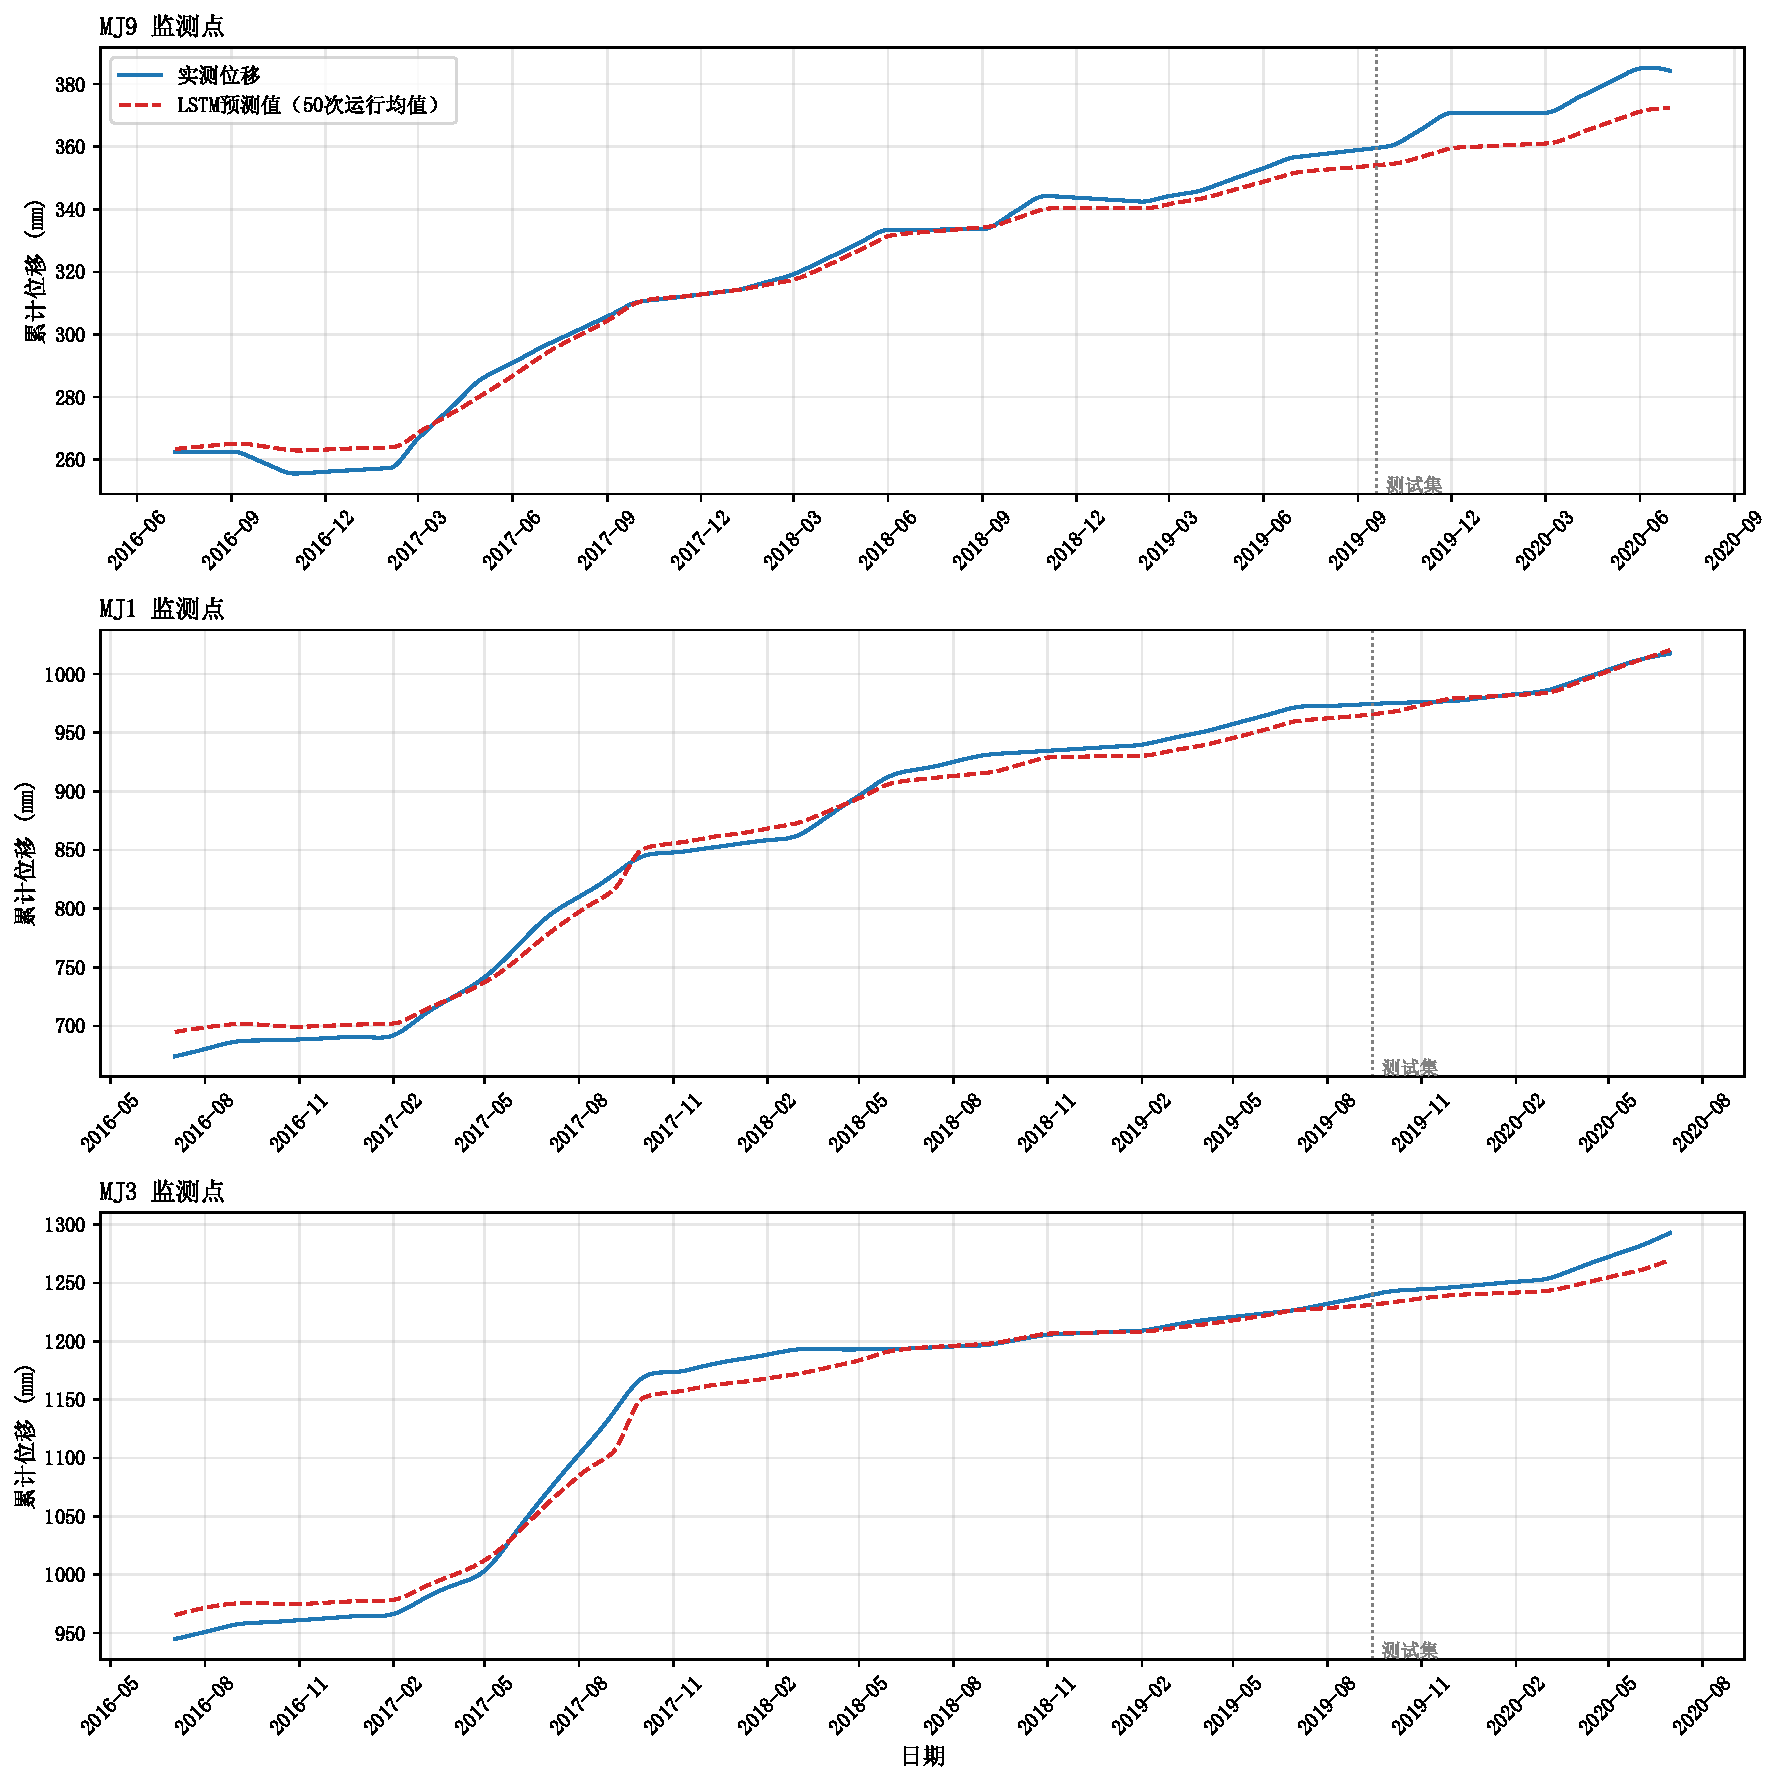
\includegraphics[width=\textwidth,height=0.58\textheight,keepaspectratio]{figures/chapter3/lstm_fitting.pdf}
    \end{column}
  \end{columns}
\end{frame}

% ============================================================
% 7. 预测结果
% ============================================================
\begin{frame}{预测结果}
  \begin{table}
    \centering
    \caption{LSTM 点预测性能（50次运行均值）}
    \begin{tabular}{lcccc}
      \toprule
      \multirow{2}{*}{监测点} & \multicolumn{2}{c}{训练集} & \multicolumn{2}{c}{测试集} \\
      \cmidrule(lr){2-3}\cmidrule(lr){4-5}
       & $R^2$ & RMSE (mm) & $R^2$ & RMSE (mm) \\
      \midrule
      MJ1 & 0.9883 & 11.02 & \alert{0.7916} & \alert{5.55} \\
      MJ9 & 0.9876 & 3.71  & $-$1.38 & 10.86 \\
      MJ3 & 0.9846 & 12.92 & 0.1124 & 13.17 \\
      \bottomrule
    \end{tabular}
  \end{table}
  \vspace{0.2em}
  \textbf{关键指标}
  \begin{itemize}
    \item MJ1 相对误差 \alert{0.56\%}，达工程应用精度；MJ9 2.86\% / MJ3 0.96\% 均可接受
    \item 三点变异系数均 $<1\%$，50次集成标准差占各自位移基线 $<1\%$，模型稳定可复现
  \end{itemize}
\end{frame}

% ============================================================
% 8. 传统预警局限与本文方法
% ============================================================
\begin{frame}{概率预警方法}
  \textbf{传统方法的局限}
  \begin{itemize}
    \item 确定性点预测：无法反映预测可信度，阈值附近频发误报/漏报
    \item 单一固定阈值：难以适应不同监测点、不同变形阶段的动态变化
  \end{itemize}
  \vspace{0.5em}
  \textbf{本文方案}
  \begin{itemize}
    \item 各监测点独立：基于自身位移统计确定基准速率 $V_0 = 1.5\bar V + 2\sigma$
    \item 50次 LSTM 预测月速率 $\to$ 统计四级概率 $\to$ 取最大概率为当日预警等级
    \item 四级划分：$V_0$（黄）$\mid$ $5V_0$（橙）$\mid$ $10V_0$（红）
  \end{itemize}
\end{frame}

% ============================================================
% 9. V0 计算与预警结果
% ============================================================
\begin{frame}{$V_0$ 阈值与预警验证}
  \begin{columns}[T]
    \begin{column}{0.45\textwidth}
      \textbf{三点 $V_0$（mm/月）}
      \begin{table}
        \centering
        \begin{tabular}{lccc}
          \toprule
          监测点 & $\bar V$ & $\sigma$ & $V_0$ \\
          \midrule
          MJ9 & 1.86 & 2.29 & 7.37  \\
          MJ1 & 6.26 & 5.56 & 20.50 \\
          MJ3 & 4.79 & 5.81 & 18.80 \\
          \bottomrule
        \end{tabular}
      \end{table}
      \vspace{0.3em}
      {\small 三点 $V_0$ 差异达 3 倍，与各点位移基线高度吻合}
    \end{column}
    \begin{column}{0.51\textwidth}
      \textbf{预警验证结果}
      \begin{itemize}
        \item \textbf{测试集盲测}（2019.7—2020.6）：三点均 \alert{100\% 特异性、零误报}
        \item \textbf{训练期阶跃段演示}（2017.7—12）：MJ1 触发 \alert{黄色预警 70 天}，MJ3 触发 \alert{129 天}
        \item 黄色预警与实测阶跃变形期显著重叠，验证方法对真实变形事件的响应能力
      \end{itemize}
    \end{column}
  \end{columns}
\end{frame}

% ============================================================
% 10. MJ1 预警时序
% ============================================================
\begin{frame}{预警时序——MJ1 监测点}
  \centering
  
\includegraphics[width=\textwidth,height=0.95\textheight,keepaspectratio]{figures/chapter4/warning_timeseries.pdf}
\end{frame}

% ============================================================
% 11. 主要结论
% ============================================================
\begin{frame}{主要结论}
  \begin{enumerate}
    \item \textbf{特征分析}：LightGBM+SHAP 定量揭示库水位消落与历史位移累积为滑坡变形主控因子，降雨、地下水位次之，气象要素贡献最小；识别最优时滞窗口（库水位 7--14 天，降雨 3--7 天）
    \item \textbf{位移预测}：多监测点 LSTM 模型 MJ1 测试集 $R^2=0.7916$，RMSE=5.55\,mm，相对误差 0.56\%，达工程应用精度；50次运行变异系数 $<1\%$，成功量化认知不确定性
    \item \textbf{概率预警}：基于 $V_0 = 1.5\bar V + 2\sigma$ 的四级动态预警体系，各监测点独立确定阈值；测试集三点均 100\% 特异性、零误报；训练期阶跃段演示中 MJ1 与 MJ3 分别触发 70 天与 129 天黄色预警，验证方法响应能力
  \end{enumerate}
  \vspace{0.3em}
  \begin{alertblock}{核心贡献}
    实现从\textbf{确定性点预测}向\textbf{概率区间预报}的转变，从\textbf{滞后性预警}向\textbf{前瞻性预警}的跨越
  \end{alertblock}
\end{frame}

% ============================================================
% 12. 致谢
% ============================================================
\begin{frame}[standout]
  \Huge 感谢各位老师！\\[0.8em]
  \large 敬请批评指正
\end{frame}

\end{document}
